

\title{Product Quality Assurance Plan}
\def \documentid {LEANOS-UVIE-PAQ-001}
\date{Issue 0.1, April 20, 2016}

\newcommand\affil[1]{\textsuperscript#1}

\def\preparedby {Armin Luntzer\affil{1}}
\def\checkedby {Roland Ottensamer\affil{1}}
\def\approvedby {Franz Kerschbaum\affil{1}}

\def\affiliations{
	\affil{1} Department of Astrophysics, University of Vienna
}




\documentclass{report}
%\usepackage[left = 2cm, right=2cm, top = 1cm]{geometry}
\usepackage[top = 2cm, bottom = 5cm]{geometry}

\usepackage[T1]{fontenc}
\usepackage{textcomp}

%\PassOptionsToPackage{table}{xcolor}


\usepackage{geometry}
\usepackage{fontspec}
%
\defaultfontfeatures[MyriadPro-SemiCondensed]{
	Path		= ../shared/fonts/,
	Extension	= .otf,
	UprightFont	= *-light,
	ItalicFont	= *-italic,
	BoldFont	= *-bold,
	BoldItalicFont	= *-bold-italic
%	LetterSpace	= 5pt		% Laufweite
}
%
\defaultfontfeatures[MyriadPro]{
	Path		= ../shared/fonts/,
	Extension	= .otf,
	UprightFont	= *-regular,
	ItalicFont	= *-italic,
	BoldFont	= *-bold,
	BoldItalicFont	= *-bold-italic
}%
\defaultfontfeatures[MyriadProLight]{
	Path		= ../shared/fonts/,
	Extension	= .otf,
	UprightFont	= MyriadPro-light,
	ItalicFont	= MyriadPro-light-italic,
}

\setmainfont{MyriadPro}



\makeatletter
\renewcommand\normalsize{%
\@setfontsize\normalsize{11pt}{14pt}
\abovedisplayskip 10\p@ \@plus2\p@ \@minus5\p@%
\abovedisplayshortskip \z@ \@plus2\p@%
\belowdisplayshortskip 5\p@ \@plus2\p@ \@minus3\p@%
\belowdisplayskip \abovedisplayskip%
\let\@listi\@listI%
}
\normalsize  
\makeatother



\usepackage{titlesec}

\titleformat{\chapter}[hang]
  {\fontspec{MyriadProLight}\fontsize{30}{36}\selectfont\color{uvie-blue}}
  {\fontspec{MyriadPro}\selectfont\thechapter.}{8pt}{}
\titlespacing*{\chapter}{0pt}{-20pt}{20pt}

\titleformat{\section}
  {\fontspec{MyriadPro}\fontsize{13}{16}\selectfont\color{uvie-blue}}
  {\thesection}{1em}{}

\titleformat{\subsection}
  {\fontspec{MyriadPro}\fontsize{13}{16}\selectfont\color{uvie-blue}}
  {\thesection}{1em}{}

\DeclareMathSizes{12}{55}{15}{15}

\usepackage[table]{xcolor}

% begin UVIE primary colours
\iffalse

% colours from numeric colour values in corporate design document
\definecolor{uvie-blue}{RGB}{0, 99, 166}
\definecolor{uvie-orangered}{RGB}{221, 72, 20}
\definecolor{uvie-goldenyellow}{RGB}{234, 171, 0}
% UVIE secondary colours
\definecolor{uvie-gray}{RGB}{102, 102, 102}
\definecolor{uvie-burgundy}{RGB}{167, 28, 73}

\else
% colours from actual colour samples in corporate design document
%r: 0 g:58 b:133
\definecolor{uvie-blue}{RGB}{0, 79, 150}
\definecolor{uvie-orangered}{RGB}{225, 55, 15}
\definecolor{uvie-goldenyellow}{RGB}{248, 169, 0}
% UVIE secondary colours
\definecolor{uvie-gray}{RGB}{104, 104, 104}
\definecolor{uvie-burgundy}{RGB}{141, 22, 51}

\fi
% end UVIE primary colours


% allowed UVIE logo height
\newlength{\maxlogoheight}\setlength{\maxlogoheight}{20mm}
\newlength{\medlogoheight}\setlength{\medlogoheight}{15mm}
\newlength{\minlogoheight}\setlength{\minlogoheight}{10mm}
%
% allowed space round logo: logoheight <= x <= 0.5 logoheight 
\def \maxlogospacing{1.0}
\def \medlogospacing{0.75}
\def \minlogospacing{0.5}

%
%elif \paperheight \equal {210mm} % A5
% todo: based on papersize: >= A4: 20mm, A5/long: 15mm, all smaller: 10mm
%\if \paperheight \equal {297mm}	  % A4
\newlength{\logoheight}{\setlength{\logoheight}{\maxlogoheight}
%elif \paperheight \equal {210mm} % A5
%\fi
%
% todo: pass as option
\newlength{\logospacing}{\setlength{\logospacing}{\medlogospacing\logoheight}


\newcommand{\fig}[1]{Figure \ref{#1}}


\newenvironment{keywords}%
   {\begin{trivlist}\item[]{\bfseries\sffamily Schlagworte:}\ }% oder "Keywords:"
   {\end{trivlist}}
%
\author{%
    Author 1 name \\
    Department name \\
    \texttt{email1@example.com}\vspace{40pt} \\
    Author 2 name \\
    Department name \\
    \texttt{email2@example.com}
    }


\usepackage{tabu}
\usepackage{colortbl}

\usepackage{array, ltxtable}
\usepackage[most]{tcolorbox}


\usepackage[some]{background}
\usepackage{tikz}
\backgroundsetup{
scale=1,
angle=0,
opacity=1,
placement=top,
contents={
	\begin{tikzpicture}[remember picture, blend mode = multiply]
		% field heights from top down: x | x | x/2 | remainder
		%
		\fill[white]		(-0.5\paperwidth,                 0.0)
							rectangle (0.5\paperwidth,       -3.0\logospacing);
		\fill[uvie-blue!75]	(-0.5\paperwidth,                -3.0\logospacing)
							rectangle (0.5\paperwidth, -2.0 * 3.0\logospacing);
		\fill[uvie-blue]	(-0.5\paperwidth,          -2.0 * 3.0\logospacing)
							rectangle (0.5\paperwidth, -2.5 * 3.0\logospacing);
		% mext can be image or colour, but must overlap with 3rd bar in multiply
		% blend mode
		% todo: make conditional on image option
		\fill[uvie-blue!75]	(-0.5\paperwidth,          -2.0 * 3.0\logospacing)
							rectangle (0.5\paperwidth,       -1.0\paperheight);
	\end{tikzpicture}}
}
%


\makeatletter
\let\doctitle\@title
\makeatother

\makeatletter
\let\docdatever\@date
\makeatother

\usepackage{fancyhdr}
\usepackage{lastpage}

\def\ifalogo{
\includegraphics[height = \medlogoheight]{../shared/images/uni_logo_astrophysik_cmyk.eps}}
\fancypagestyle{plain}{ % call style plain so it is used by chapter pages as well
	\fancyhf{}
	\fancyhead[R]{
		\fontspec{MyriadPro}\docdatever \\
		\vspace{2em}
		Page \thepage\ of \pageref*{LastPage} 
	}

	\fancyhead[C]{
		{
			\fontspec{MyriadPro}
			\documentid \\
			\vspace{.7em}
			\doctitle
			\vspace{.9em}
		}
	}
	\fancyhead[L]{
		\ifalogo%
	}
}
\setlength\headheight{80pt}
\pagestyle{plain}


% def \preparedby, \checkedby, \approvedby, \documentid, \docdatever, \doctitle
\def\approvalpage{
	\clearpage
	\pagestyle{empty}
	\null
	\vfil

	{\fontspec{MyriadPro}\fontsize{20}{24}\selectfont\color{uvie-blue}
	 \doctitle}

	\vspace*{1\baselineskip}

	\begin{tabular}{@{}ll}
		\textbf{Reference:}   & \documentid \\[2ex]
		\textbf{Version:}     & \docdatever \\[6ex]
		\textbf{Prepared by:} & \preparedby \\[1ex]
		\textbf{Checked by:}  & \checkedby  \\[1ex]
		\textbf{Approved by:} & \approvedby \\[1ex]
	\end{tabular}

	\vspace*{0.5\baselineskip}
	{\footnotesize \affiliations}


	\vfill

	\begin{minipage}[b]{0.9\textwidth}
	\footnotesize\raggedright
	\setlength{\parskip}{0.5\baselineskip}
	Copyright \copyright \the\year\ \par
	Permission is granted to copy, distribute and\slash or modify this
	document under the terms of the GNU Free Documentation License,
	Version 1.3 or any later version published by the Free Software
	Foundation; with no Front-Cover, no Logos of the University of Vienna.
	\end{minipage}
	\vspace*{2\baselineskip}
	\cleardoublepage

	\pagestyle{plain}
}

\newcommand{\uvietitlepage}[3]{%
\begin{titlepage}
\BgThispage
%
%
\begin{tikzpicture}[overlay, remember picture]
\node[anchor	= north west,
      xshift	= \logospacing,
      yshift	=-\logospacing] 
      at (current page.north west)
     {
\includegraphics[height = \logoheight]{../shared/images/uni_logo_astrophysik_cmyk.eps}}; 
\end{tikzpicture}
%
\begin{tikzpicture}[overlay, remember picture]
\node[anchor	= north east,
      xshift	=-\logospacing,
      yshift	=-\logospacing] 
      at (current page.north east)
     {
\includegraphics[height = \logoheight]{../shared/images/uni_logo_farbe_02.eps}}; 
\end{tikzpicture}
%
%
%
% main title, must not exceed 3 lines 
\begin{tikzpicture}[overlay, remember picture]
\node[anchor			= north west,
      xshift			= \logospacing,
      yshift			=-\logospacing * 3.0,
	  minimum height	= \logospacing * 3.0,
	  text width		= \textwidth]
      at (current page.north west)
      {\fontsize{30pt}{36pt}\selectfont
       \textcolor{white}
       {
			\uppercase{#1}
       }
       \par
      };
\end{tikzpicture}
%
% subtitle, must not exceed 3 lines 
\begin{tikzpicture}[overlay, remember picture]
\node[anchor			= north west,
      xshift			= \logospacing,
      yshift			=-\logospacing * 5.5,
	  minimum height	= \logospacing * 2.5,
	  text width		= \textwidth]
      at (current page.north west)
      {\fontsize{13pt}{16pt}\selectfont
       \textcolor{white}
       {
			\uppercase{\textbf {#2}}
       }
       \par
      };
\end{tikzpicture}
%
%\noindent
%\hfill
% \hspace*{-3cm}
\begin{tikzpicture}[overlay, remember picture]
\node[anchor=south east,		%anchor is upper left corner of the graphic
      xshift  = 0.5cm,		%shifting around
      yshift  = -0.5cm] 
     	at (current page.south east) %left upper corner of the page
     {\includegraphics[width=14.0cm]{#3}}; 
\end{tikzpicture}
%
%
\end{titlepage}
%
\restoregeometry
%
\newpage
}% newcommand uvietitlepage


\usepackage{xintexpr, xinttools}

\usepackage{xr-hyper} % load before hyperref
\usepackage{hyperref}% check if ok with hyperlinks
\hypersetup{colorlinks=true, linkcolor=uvie-blue}

\usepackage{xifthen}
\usepackage{pifont}
\usepackage{adjustbox}	% \rot

\usepackage{stringstrings}


\newcommand{\requirements}{}
\newcommand{\designs}{}
\providecommand*\phantomsection{}

\makeatletter

\newcommand{\req}[1]{%
	\textbf{R-#1}%
	\phantomsection
	\def\@currentlabel{R-#1}%
	\label{req@#1}%
  	\@ifundefined {req@#1} {%
  		\global\@namedef{req@#1}{}%
  		\g@addto@macro\requirements{{req@#1}}%
	}{}%
}

\newcommand{\reqgoal}[1]{%
	\textbf{G-#1}%
	\phantomsection
	\def\@currentlabel{G-#1}%
	\label{req@#1}%
	\@ifundefined {req@#1} {%
		\global\@namedef{req@#1}{}%
		\g@addto@macro\requirements{{req@#1}}%
	}{}%
}

\newcommand{\meetsthisreq}[1]{% (renamed from \meetsreq above)
  \@ifundefined {req@#1@ismetby} {%
  \global\@namedef{req@#1@ismetby}{}%
  }{}% this is called multiple times when creating a table, generate only one
  \ref{REQ-req@#1}%
  \expandafter\g@addto@macro\csname req@#1@ismetby\expandafter\endcsname 
              \expandafter {\expandafter{\@currentdesign}}%
}

\newcommand{\meetsreq}[1]{% (handles comma separated list)
  \xintListWithSep{, }{\xintApply{ \meetsthisreq}{\xintCSVtoList{#1}}}%
}



\newcommand{\designswithreq}[1]% 
% The space before \ref below is intentional and will be swallowed by \xintApply
% It is not mandatory however, the thing works without it too.
 {\csname #1@ismetby\endcsname}

\newcommand{\designswithreqref}[1]% 
% The space before \ref below is intentional and will be swallowed by \xintApply
% It is not mandatory however, the thing works without it too.
 {\xintListWithSep{, }{\xintApply { \ref}{\csname #1@ismetby\endcsname }}}

\newcommand{\newdesign}[1]{%
  	\textbf{D-#1}%
  	\phantomsection
  	\def\@currentlabel{D-#1}%
	\label{design@#1}%
  	\@ifundefined {design@#1} {%
  		\global\@namedef{design@#1}{}%
		\gdef\@currentdesign{design@#1}%
  	\g@addto@macro\designs{{design@#1}}%
	}{}
}


\newcommand{\design}[5]{%
	\rowcolors{1}{white}{white}%
	\begin{tcolorbox}[enhanced, notitle, clip upper,%
			  sharp corners, colframe = white, colback = white,%
		tabularx={%
						  p{0.15\columnwidth}%
				>{\arraybackslash\raggedright}p{0.10\columnwidth}%
				>{\arraybackslash}X%
			}%
		]%
	%
	\vspace{-.65\baselineskip}	% uuuaaahhh..why? :(
	\cellcolor{uvie-blue!75}\color{white}\newdesign{#1} &%
	\vspace{-.65\baselineskip}%
	\cellcolor{uvie-blue!50}\color{white}\textbf{Identifier} &%
	\vspace{-.65\baselineskip}%
	\cellcolor{uvie-blue!50}\color{white}\textbf{Function} \\%
	& #2 & #3%

	\\%
	\vspace{-1em}%
	\arrayrulecolor{uvie-blue!75}\renewcommand{\arraystretch}{1.2}
	\color{uvie-blue!75}\textbf{Purpose} &%
	\multicolumn{2}{|>{\arraybackslash\raggedright}X}{#4}%

	\ifthenelse{\isempty{#5}} {}{%
		\\%
		\vspace{-1em}%
		\arrayrulecolor{uvie-blue!75}\renewcommand{\arraystretch}{1.2}
		\color{uvie-blue!75}\textbf{Comment} &%
		\multicolumn{2}{|>{\arraybackslash}X}{#5}%
	}%
	\vspace{1em}
	\end{tcolorbox}%
}





\newcommand{\requirement}[4]{%
	\rowcolors{1}{white}{white}%
	\begin{tcolorbox}[enhanced, notitle, clip upper,%
			  sharp corners, colframe = white, colback = white,%
		tabularx={%
						  p{0.15\columnwidth}%
				>{\arraybackslash\raggedright}p{0.15\columnwidth}%
				>{\arraybackslash}X%
			}%
		]%
	%
	\vspace{-.65\baselineskip}	% uuuaaahhh..why? :(
	\cellcolor{uvie-blue!75}\color{white}\req{#1} &%
	\vspace{-.65\baselineskip}%
	\cellcolor{uvie-blue!50}\color{white}\textbf{Short Text} &%
	\vspace{-.65\baselineskip}%
	\cellcolor{uvie-blue!50}\color{white}\textbf{Software Requirement} \\%
	& #2 & #3%

	\ifthenelse{\isempty{#4}} {}{%
		\\%
		\vspace{-1em}%
		\arrayrulecolor{uvie-blue!75}\renewcommand{\arraystretch}{1.2}%
		\color{uvie-blue!75}\textbf{Comment}&%
		\multicolumn{2}{|>{\arraybackslash}X}{#4}%
	}%
	\vspace{1em}
	\end{tcolorbox}%
}



\newcommand{\goal}[4]{%
	\rowcolors{1}{white}{white}%
	\begin{tcolorbox}[enhanced, notitle, clip upper,%
			  sharp corners, colframe = white, colback = white,%
		tabularx={%
						  p{0.15\columnwidth}%
				>{\arraybackslash}p{0.2\columnwidth}%
				>{\arraybackslash}X%
			}%
		]%
	%
	\vspace{-.65\baselineskip}	% uuuaaahhh..why? :(
	\cellcolor{uvie-gray!75}\color{white}\reqgoal{#1} &%
	\vspace{-.65\baselineskip}%
	\cellcolor{uvie-gray!50}\color{white}\textbf{Short Text} &%
	\vspace{-.65\baselineskip}%
	\cellcolor{uvie-gray!50}\color{white}\textbf{Software Requirement} \\%
	& #2 & #3%
	\ifthenelse{\isempty{#4}} {}{%
		\\%
		\vspace{-1em}%
		\arrayrulecolor{uvie-gray!75}\renewcommand{\arraystretch}{1.2}
		\color{uvie-gray!75}\textbf{Comment} &%
		\multicolumn{2}{|>{\arraybackslash}X}{#4}%
	}%
	\vspace{1em}
	\end{tcolorbox}%
}





\newcommand{\exportrequirements}{%
\AtEndDocument{%
	\newwrite\reqfile
	\immediate\openout\reqfile=requirements.list
	\immediate\write\reqfile{\string\renewcommand{\string\requirements}{\requirements}}
	\immediate\closeout\reqfile
}}%


\makeatletter


\newcommand*\traceabilitymatrix[]{%
%
	\newcommand{\numitems}[1]{{\expandafter\xintLength\expandafter{##1}}}%
	\newcommand*\OK{\ding{51}}%
%
	\newcounter{numdesigns}%
	\setcounter{numdesigns}{\numitems{\designs}}%
	\stepcounter{numdesigns}%
%
	\newcommand*\rot{\multicolumn{1}{R{90}{0em}}}%
%
	%\begin{table}[h]
	\newcolumntype{C}{>{\centering\arraybackslash} m{0.2cm}}%
	\newcolumntype{R}[2]{>{\adjustbox{angle=##1,lap=\width-(##2)}\bgroup}l<{\egroup}}%
	\rowcolors{1}{uvie-gray!25}{white}%
	\begin{longtable}{c*{\value{numdesigns}}CC} %+1 linespacing column
	\xintFor* ##1 in \designs \do {%
		&  \rot{\fontspec{MyriadPro}\fontsize{8}{9}\ref{##1}\,\,\normalfont}%
	} \\%
	\endhead
	% it's hilariously inefficient, faster methods are welcome...
	\xintFor* ##1 in \requirements \do {%
	% TODO: recolor link if goal
	%	\isnextbyte[q]{R}{\string\ref{##1}} \par
	%	\if T\theresult moopp\hypersetup{filecolor=uvie-burgundy}\fi

		\fontspec{MyriadPro}\fontsize{8}{9}\ref{REQ-##1}\normalfont %
		\hypersetup{filecolor=uvie-blue}
		\xintFor* ##2 in \designs \do {%
			&%
			\xintFor* ##3 in {\designswithreq{##1}} \do {%
				\ifthenelse{\equal{##2}{##3}} {%
					\cellcolor{uvie-blue!50}%
					%\OK
					\xintBreakFor%
				}{}%
			}%
		}\\[0.1cm]%
	}%
	\end{longtable}%
	%\end{table}%
}%


\usepackage{stringstrings}

\def\rereadauxdesignlabels{
	\newtoks\designlist%
	\newread\zz%
	\immediate\openin\zz=\jobname.aux%
	\loop%
	\ifeof\zz\else%
	\read\zz to \tmp%
	\expandafter\findlabeldesign\tmp\relax\findlabel%
	\repeat%
}


\long\def\findlabeldesign#1#2\findlabel{%
 \ifx\newlabel#1\designlist\expandafter{\the\designlist\showlabeldesign#2}\fi}


%hyperref has 4 felds in each label could use them but don't here
\def\showlabeldesign#1#2{%
	%\begin{minipage}{\textwidth}%
	\findwords[q]{\expandafter\string\detokenize{#1}}{design}%
		\ifnum\theresult>0%
		\par\noindent\ref{#1}\dotfill\pageref{#1}%
		\fi%
	%\end{minipage}%
}


\def\rereadauxrequirementlabels{
	\newtoks\requirementlist
	\newread\zz
	\immediate\openin\zz=\jobname.aux
	\loop
	\ifeof\zz\else
	\read\zz to \tmp
	\expandafter\findlabelrequirement\tmp\relax\findlabel
	\repeat
}


\long\def\findlabelrequirement#1#2\findlabel{%
 \ifx\newlabel#1\requirementlist\expandafter{\the\requirementlist\showlabelrequirement#2}\fi}

\newsavebox{\fminipagebox}
\NewDocumentEnvironment{fminipage}{m O{\fboxsep}}
 {\par\kern#2\noindent\begin{lrbox}{\fminipagebox}
  \begin{minipage}{#1}\ignorespaces}
 {\end{minipage}\end{lrbox}%
  \makebox[#1]{%
    \kern\dimexpr-\fboxsep-\fboxrule\relax
    \fbox{\usebox{\fminipagebox}}%
    \kern\dimexpr-\fboxsep-\fboxrule\relax
  }\par\kern#2
 }


%hyperref has 4 felds in each label could use them but don't here
\def\showlabelrequirement#1#2{%
	\begin{minipage}{\textwidth}%
	\findwords[q]{\expandafter\string\detokenize{#1}}{req}%
		\ifnum\theresult>0%
		\par\noindent\ref{#1}\dotfill\pageref{#1}%
		\fi%
	\end{minipage}%
}

\usepackage[xindy, nopostdot, numberedsection, style=super, section, toc, acronyms, nogroupskip]{glossaries}
\usepackage{xparse}

\setlength{\glsdescwidth}{0.8\textwidth}
\renewcommand{\glsnamefont}[1]{\textbf{#1}}

% label, acronym, name, description
\DeclareDocumentCommand{\newdualentry}{ m m m m } {
	\newglossaryentry{gls-#1}{
	name={#3 (\gls{#1})},
	description={#4}, nonumberlist
	}
	\newglossaryentry{#1}{
		type=\acronymtype,
		name={#2},
		first={#3 (#2)},
		firstplural={#3s (#2s)},
		see={[Glossary:]{\gls{gls-#1}}},
		description=\glslink{gls-#1}{#3},
		nonumberlist
	}%
}
%%% \gls{ABBREV} to point at Acronym/Abbreviation index
%%% \gls{gls-ABBREV} to point to glossary


\newdualentry{ADC}%
  {ADC}%
  {Analog to Digital Converter}%
  {An Analog to Digital Converter is a system that converts an analog signal
   into a quantized digital signal. Its counterpart is the \gls{DAC}.}%

\newdualentry{API}%
  {API}%
  {Application Programming Interface}%
  {The Application Programming Interface defines how a developer can write
   a program that requests services from an operating system or application.
   \glspl{API} are implemented by function calls composed of verbs and nouns,
   i.e. a function to execute on an object.}%

\newdualentry{BSP}%
  {BSP}%
  {Board Support Package}%
  {A Board Support Package is the implementation of a specific interface defined
   by the abstract layer of an operating system that enables the latter to run
   on the particular hardware platform.}%

\newdualentry{CPU}%
  {CPU}%
  {Central Processing Unit}%
  {The Central Processing Unit is the electronic circuitry that interprets
  instructions of a computer program and performs control logic, arithmetic,
  and input/output operations specified by the instructions. It maintains
  high-level control of peripheral components, such as memory and other devices.}%

\newdualentry{DAC}%
  {DAC}%
  {Digital to Analog Converter}%
  {A Digital to Analog Converter is a system that converts a quantized digital
   signal into an analog signal. Its counterpart is the \gls{ADC}.}%

\newdualentry{DMA}%
  {DMA}%
  {Direct Memory Access}%
  {Direct Memory Access is a feature of a computer system that allows hardware
   subsystems to access main system \gls{gls-RAM} directly, thereby bypassing
   the \gls{gls-CPU}.}%

\newdualentry{DSP}%
  {DSP}%
  {Digital Signal Processor}%
  {A Digital Signal Processor is a specialised processor with its architecture %
   targeting the operational needs of digital signal processing.}%

\newdualentry{ELF}%
  {ELF}%
  {Executable and Linkable Format}%
  {The Executable and Linkable Format is a common standard file format for
   executables, object code, shared libraries, and core dumps.}%

\newdualentry{FIFO}%
  {FIFO}%
  {First In - First Out}%
  {In FIFO processing, the "head" element of a queue is processed first.
   Once complete, the element is removed and the next element in line becomes
   the new queue head.}%

\newdualentry{FPU}%
  {FPU}%
  {Floating Point Unit}%
  {A co-processor unit that specialises in floating-point calculations.}%

\newdualentry{ILP}%
  {ILP}%
  {Instruction Level Parallelism}%
  {Instruction-level parallelism (ILP) is a measure of how many instructions in
   a computer program can be executed simultaneously by the \gls{CPU}.}%

\newdualentry{ISR}%
  {ISR}%
  {Interrupt Service Routine}%
  {An Interrupt Service Routine is a function that handles the actions needed
   to service an interrupt.}%

\newdualentry{GCC}%
  {GCC}%
  {GNU Compiler Collection}%
  {The GNU Compiler Collection is a compiler system produced by the
   GNU project. It is part of the GNU toolchain collection of programming
   tools.}%

\newglossaryentry{GNU}{
  name={GNU},
  description={GNU is a recursive acronym that stands for "GNU's Not Unix!".
	      The GNU project is a free software collaboration project announced
	      in 1987. Users are free to run GNU-licensed software, share, copy,
	      distribute, study and modify it. GNU software guarantees these
	      freedom-rights legally via its license and is thefore free
      	      software.},
  nonumberlist
}

\newglossaryentry{LEON2}{
  name={LEON2},
  description={The LEON2 is a synthesisable VHDL model of a 32-bit processor
	       compliant with the SPARC V8 architecture. It is highly
	       configurable and particularly suitable for \gls{SoC} designs.
	       Its source code is available under the GNU LGPL license},
  nonumberlist
  }

\newglossaryentry{LEON3}{
  name={LEON3},
  description={The LEON3 is an updated version of the \gls{LEON2}, changes
	       include \gls{gls-SMP} support and a deeper instruction pipeline},
  nonumberlist
  }

\newglossaryentry{LEON3-FT}{
  name={LEON3-FT},
  description={The LEON3-FT is a fault-tolerant version of the \gls{LEON3}.
  	       Changes to the base version include autonomous error handling,
       	       cache locking and different cache replacement strategies.},
  nonumberlist
  }

\newdualentry{MMU}%
  {MMU}%
  {Memory Management Unit}%
  {A Memory Management Unit performs address space translation between physical
   and virtual memory pages and protects unprivileged access to certain memory
   regions.}%

\newdualentry{MPPB}%
  {MPPB}%
  {Massively Parallel Processor Breadboarding system}%
  {The Massively Parallel Processor Breadboarding system is a proof-of-concept %
   design for a space-hardened, fault-tolerant multi-DSP system with various %
   subsystems to build a powerful digital signal processing system with a high %
   data throughput. Its distinguishing features are the \gls{gls-NoC} and the
   \gls{Xentium} \glspl{DSP} controlled by a \gls{LEON2} processor.
   It was developed under ESA contract 21986 by Recore Systems B.V.}%

\newdualentry{NGAPP}%
  {NGAPP}%
  {Next Generation Astronomy Processing Platform}%
  {Next Generation Astronomy Processing Platform was an evaluation of the
   \gls{MPPB} performed in a joint effort of RUAG Space Austria and the
   Department of Astrophysics of the University of Vienna.
   The project was funded under ESA contract 40000107815/13/NL/EL/f.}%

\newdualentry{NoC}%
  {NoC}%
  {Network On Chip}%
  {A Network On Chip is a communication system on an integrated circuit that
   applies (packet based) networking to on-chip communication. It offers
   improvements over more conventional bus interconnects and is more scalable
   and power efficient in complex \gls{gls-SoC} desgins.}%

\newdualentry{POSIX}
  {POSIX}
  {Portable Operating System Interface}
  {The Portable Operating System Interface is a family of standards specified
   by the IEEE Computer Society for maintaining compatibility between
   operating systems.}%

\newdualentry{PUS}
  {PUS}
  {Packet Utilisation Standard}
  {The Packet Utilisation Standard addresses the end-to-end transport of telemetry
   and telecommand data between user applications on the ground and applications
   onboard a satellite. See also ECSS-E-70-41A.}%

\newdualentry{RAM}%
  {RAM}%
  {Random-Access Memory}%
  {Random-Access Memory is a type of memory where each memory cell may be
   accessed directly via their memory addresses.}%

\newdualentry{RISC}%
  {RISC}%
  {Reduced Instruction Set Computing}%
  {RISC is a \gls{CPU} design strategy that intends to improve performance by
   combining a simplified instruction set with a microprocessor architecture
   that is capable of executing an instruction in a smaller number of clock
   cycles.}%

\newdualentry{RMAP}%
  {RMAP}%
  {Remote Memory Access Protocol}%
  {The Remote Memory Access Protocol is a form of \gls{SpaceWire} communication
   that transparently communicates writes to memory mapped regions between
   different hardware devices.}%


\newdualentry{RR}%
  {RR}%
  {Round Robin}%
  {Round Robin is a scheduling algorithm where time slices are assigned in equal
   poritions and in circular order. In the context of threads, priorities are
   usually only used to control re-scheduling order when a mutex is accessed by
   a thread.}%

\newacronym{RSA}{RSA}{RUAG Space Austria}

\newdualentry{SMP}%
  {SMP}%
  {Symmetric Multiprocessing}%
  {Symmetric Multiprocessing denotes computer architectures, where two or more
   identical processors are connected to the same periphery and are controlled
   by the same operating system instance.}%

\newdualentry{SoC}%
  {SoC}%
  {System On Chip}%
  {A System On Chip is an integrated circuit that combines all components of a %
   computer or other electronic system into a single chip.}%

\newglossaryentry{SpaceWire}{
  name={SpaceWire},
  description={SpaceWire is a spacecraft communication network based in part
               on the IEEE 1355 standard of communications.},
  nonumberlist
  }

\newglossaryentry{SPARC}{
  name={SPARC},
  description={SPARC ("scalable processor architecture") is a \gls{gls-RISC}
  	       instruction set architecture developed by Sun Microsystems in
	       the 1980s. The distinct feature of SPARC processors is the high
	       number of \gls{gls-CPU} registers that are accessed similarly to
	       stack variables via ``sliding windows''.},
  nonumberlist
  }

\newdualentry{SSDP} % label
  {SSDP}            % abbreviation
  {Scalable Sensor Data Processor}  % long form
  {The Scalable Sensor Data Processor (SSDP) is a next generation on-board %
   data processing mixed-signal ASIC, envisaged to be used in future scientific %
   payloads requiring high-performance on-board processing capabilities. %
   It is built opon a heterogeneous multicore architecture, combining two %
   \gls{Xentium} \gls{DSP} cores with a general-purpose \gls{LEON3-FT} control %
   processor in a \gls{gls-NoC}.} % description


\newdualentry{TCM}%
  {TCM}%
  {Tightly-Coupled Memory}%
  {Tightly-Coupled Memory is the local data memory that is directly accessible %
   by a Xentium's load/store unit. It can be viewed as a completely %
   program-controlled data cache.}%


\newacronym{UVIE}{UVIE}{University of Vienna}

\newdualentry{VLIW}%
  {VLIW}%
  {Very Long Instruction Word}%
  {Very Long Instruction Word is a processor architecture design concept that
   exploits \gls{gls-ILP}. This approach allows higher performance at a smaller
   silicone footprint compared to serialised instruction processors, as no
   instruction re-ordering logic to exploit superscalar capabilities of the
   processor must be integrated on the chip, but requires either code to be
   tuned manually or a very sophisticated compiler to exploit the full potential
   of the processor.}%

\newglossaryentry{Xentium}{
  name={Xentium},
  description={The Xentium is a high performance \gls{gls-VLIW} \gls{DSP} core.
               It operates 10 parallel execution slots supporting 32/40 bit
	       scalar and two 16-bit element vector operations.},
  nonumberlist
  }


% do not remove
\glsresetall
\makeglossaries

 
\usepackage{multicol}
\usepackage{enumitem}
\usepackage{vhistory}

\usepackage{biblatex}
\addbibresource{../shared/bibliography.bib}




\begin{document}


\setmainfont{MyriadPro-SemiCondensed}
\uvietitlepage%
{Lean OS --\\ An operating system for the SSDP}%
{\doctitle}%
{../shared/images/logo2.pdf}
\setmainfont{MyriadPro}

\approvalpage

\tableofcontents
\newpage



\begin{versionhistory}
  \vhEntry{0.1}{20.04.2016}{AL}{Initial version}
\end{versionhistory}


\chapter{Introduction}

\section{Purpose of the Document}


This document describes the \gls{SQA} activities that will be
performed in the development of the the operating system kernel LeanOS.
The document is applicable for all versions of LeanOS and and shall be updated
as needed.\\

\noindent
LeanOS targets the \gls{SSDP}, and to a lesser extent, its
compatible predecessor, the \gls{MPPB} v2.x \cite{MPPB}.
It is intended to be used in unmanned space applications of at least
Software Criticality Level C. \\

\noindent
This document follows the document structure for software product assurance
plans found in Annex B of ECSS-Q-ST-80C \cite{ECSS80C}.


\chapter{Applicable and Reference Documents} % does not break automatically for some reason

\printbibliography[heading=none]


\chapter{Terms, Definitions and Abbreviated Items}
\printglossary[type=acronym]
\printglossary[type=main, style=altlist]


\chapter{System Overview}

In the course of the \gls{NGAPP} activities, an evaluation of the \gls{MPPB}
was performed in a joint effort of \gls{RSA} and the Department of Astrophysics
of the \gls{UVIE}. While the original intent of the work of \gls{UVIE} was to
quantify the performance of the \gls{Xentium} \glspl{DSP} and the \gls{MPPB} as a
whole with regard to on-board data treatment and reduction in an astronomical
mission setting, it was found that, given the highly innovative nature of this new
processing platform, a novel approach was needed concerning the management of
system resources, \gls{DMA} mechanics and \gls{DSP} program design for best
efficiency and turnover rates. Consequently, \gls{UVIE} developed an experimental
operating system to stably drive the \gls{DSP} cores and the \gls{MPPB} close
to its performance limit. LeanOS is a development based on this operating system
concept.\\

\noindent
Further details on LeanOS may be found in \cite{ssdpOS}.


\chapter{Software Product Assurance Programme Implementation}

\section{Organisation}

\begin{figure}[htb]
\begin{center}
	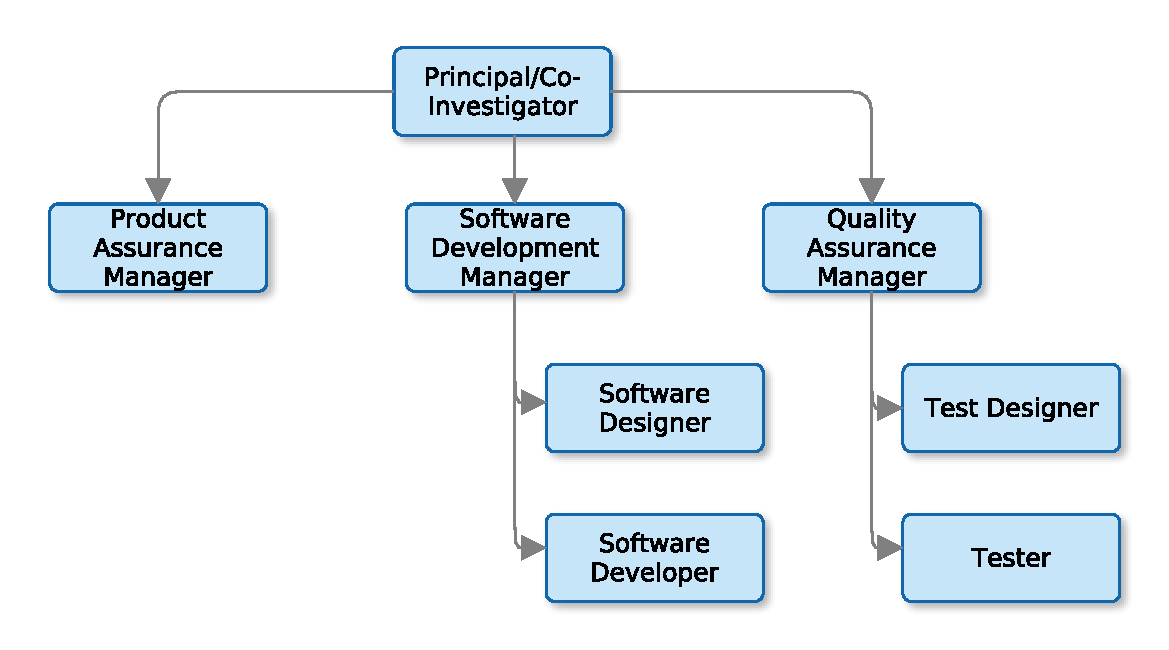
\includegraphics[width=0.7\columnwidth]{images/software_dev_structure}
	\caption{A typical organisational structure in a software development
		 group.}
	\label{fig:sw_dev_org}
\end{center}
\end{figure}

\noindent
The \gls{SQA} organisation (\fig{fig:sw_dev_org}) for the development of LeanOS
is commensurate to the scope and size of the working group dedicated to
\gls{FSW} development at the Department of Astrophysics of the University of
Vienna.\\

\noindent
As projects are typically carried out by a small group of people, several of
the project tasks may be executed by one and the same person.\\

\noindent
There is no formal \gls{PA} section at the Department of Astrophysics.
Instead, the \gls{PAM}, together with the other team leaders, forms a \gls{PA}
group for the specific project. In particular, the \gls{PAM} also takes over the
role of the \gls{SQAM} and nominates people as \gls{SQ} personnel as needed
and if applicable.\\

\noindent
\gls{PAM} and (internal) \gls{SQ} personnel maintain a level of independence
from the project and the software development.



\section{Responsibilities}

Formal responsibilities of the \gls{PAM} and \gls{SQ} personnel include process
and product assessments:

\begin{itemize}
	\item System and System Design Reviews
	\item Requirements Management
	\item Test Management
	\item \gls{NCR} Manangement
	\item \gls{SPR} Manangement
	\item Document Reviews and Review Packages
	\item Software Development Records
	\item Software Configuration Management
\end{itemize}

\noindent
Given the organisational and personnel constraints described in the previous
sections, activities of the \gls{SQ} personnel shall be conducted in an informal
way between the members. The \gls{PAM} shall assess and give assistance as to
the formal aspects of the product and process assurance. Examples of this
are configuration management or the state of completeness of review packages.\\

\noindent
The \gls{PAM} ensures the compliance with the software development processes
described in the corresponding software development plan if applicable.\\

\noindent
The main responsibilities of \gls{SQA} shall remain with the project team, in
particular the relevant software developer. In particular, this concerns
the documentation of any findings from software related activities, e.g. bug
tracking and repeated software testing during the development cycle.



\section{Resources}

Staffing to support software assurance activities must be balanced against the
other activities that are to be carried out within the project at any given time
period and against underlying availability of personnel.

The required resource levels shall be discussed, adjusted and managed in
conjunction with project management to ensure maintainance of adequate support
within the life cycle of the project.


\section{Reporting}

Since the project is not concerned with external partners, reporting is done
informally, rather than via \glspl{SPAMR}.\\

\noindent
Still, these informal reports shall cover:

\begin{itemize}
	\item \gls{SSS} coverage
	\item \gls{SRS} coverage
	\item \gls{SDD} coverage
	\item Testing activities
	\item Verification activities
	\item \gls{NCR} and action status
	\item \gls{SPR} and action status
	\item Product metrics
	\item Compliance and adherance to design and coding standards
	\item Methods and tooling
\end{itemize}

\noindent
No minutes of meeting or other record has to be made of meetings regarding
these informal reports.


\section{Quality models}

In ECSS-Q-ST-80C\cite{ECSS80C}, these potential quality characteristics of a
software application are identified:

\begin{multicols}{2}
\begin{itemize}
	\item functionality
	\item reliability
	\item maintainability
	\item reusability
	\item suitability for safety
	\item security
	\item usability
	\item efficiency
	\item portability
	\item software development effectiveness
\end{itemize}
\end{multicols}

\noindent
Functionality is explicitly covered in the \gls{SRS}\cite{leanosSRS}. Similarly,
the \gls{SRS} also covers maintainability, safety and security requirements, as
well as efficiency.\\

\noindent
Reliability is covered implicitly through the requirements formulated in the
\gls{TP}\cite{leanosTP} and \gls{TS}\cite{leanosTS}. which are designed to
to demonstrate the ability of the software to satisfy its requirements within
its operational domain.\\

\noindent
Usability is not formally relevant for LeanOS, but rather implied by software
design and its intended application.\\

\noindent
Portability and reusability are implicity by the type of software product
(an embedded operating system).\\

\noindent
Software development effectiveness is not covered explicitly, but is implicitly
covered by the definition of the development process.


\section{Risk Management}

If software-specific risks are identified during development, they shall be
incorporated into a risk portfolio by the \gls{PAM}. The status of corrective
and/or preventive actions shall be tracked, including a a general action plan
and progress per identified risk.\\

Given the small group of involved personnel, communication is straightforward
and ensures an efficient flow of information on an informal level.


\section{Supplier selection and control}

\emph{Not applicable.}


\section{Methods and tools}

The following tools are used for the management process:

\begin{description}[labelwidth=4em,leftmargin=\parindent,labelindent=\parindent]
	\item[\textbf{git}]		source code and document version control
	\item[\textbf{TeX Live}]	document preparation
\end{description}


\noindent
The following tools are used for the software development and testing process:

\begin{description}[labelwidth=4em,leftmargin=\parindent,labelindent=\parindent]
	\item[\textbf{sparc-gcc}]	C language compiler for \gls{SPARC}
	\item[\textbf{xentium-clang}]	C language compiler for the \gls{Xentium}
	\item[\textbf{gcov}]		code coverage testing
	\item[\textbf{doxygen}]		in-line software and \gls{API} documentation
\end{description}

\noindent
All of the listed tools are well established and are at a high level of maturity.


\section{Process assessment and improvement}

Assessment and possible improvement of the development process shall be done 
internally on an informal basis.


\section{Operations and maintenance}

No special quality measures are defined for operations or maintenance.



\chapter{Software Process Assurance}


\section{Software development cycle}

For the software development life cycle, the \emph{Agile} model is selected to
be used for the development of LeanOS.
This model keeps the initial planning and analysis is to a very high level, that
is just detailed enough to outline the scope of the project. The development
process is a series of iterations, in which a feature is taken from start to
finish during a single iteration and released intermediately during or at the
end of an iteration. There are no distinct stages during a cycle, but activities
such as analyzing, designing, developing and testing of a feature are executed
in turn within each iteration.
The benefit of this approach is the freedom to quickly and flexibly react to
changing circumstances such as changes to hardware features of the underlying
platform, or evolving use cases for the software product. Changes can be
discussed and new features can be implemented or those with shortcomings removed
or replaced, based on feedback of the user base. However, since this type of
work requiress experienced developers that are capable of independent decision
making and a wide skill set that covers efficient design and implementation, as
well as thorough test conception, adequate personnel must be carefully selected
for staffing.



\section{Project plans}

A \glsdesc{TP} is given in \cite{leanosTP}.


\section{Software dependability and safety}

LeanOS is intended to be used is intended to be used in unmanned space
applications of at least Software Criticality Level C. However, \gls{FDIR}
analyses and derived measures, as well as the particular configuration of
the operating system to be used is highly dependent on the use case and must
be defined at a different stage. Fundamental dependability on a software
component level is ensured by verification and validation testing as part of the
software development process.


\section{Software documentation and configuration management}

Documents are written and typeset in \LaTeX\ and compiled with the \textbf{TeX Live}
distribution of tools. For configuration management of both documents and source
code, \textbf{git} is used, which provides implicit protection of software and
document versions by cryptographic means.\\

\noindent
Document identification, content, change records and issue/revision handling
shall be oriented along the applicable \gls{DRD} of the corresponding ECSS
standards.\\

\noindent
The \gls{PAM} shall verify any documentation before release as to formal
standards, such as document identifier, completeness of information, date,
issue and revision.\\

\noindent
As part of the preparation of a documentation package for external review, both
the project manager and the \gls{PAM} shall perform a full review of the
contained documentation.\\

\noindent
All released documents, unless otherwise marked, can be considered signed, even
without the inclusion of an actual signature.\\

\noindent
Nonconformance management and closure processes shall follow the procedures
outlined in \cite{ECSS80C} and \cite{ECSSQ1009C} if needed when dealing with
external partners. Internally, \glspl{NCR} are handled informally, no \gls{NRB}
is foreseen to be instated.


\section{Process metrics}

Actions, \glspl{NCR}, \glspl{SPR}, resulting deviations and waivers, as
well as \gls{SQA} statistics shall be managed by the \gls{SQAM} as applicable.
No formal method of how records are kept is specified.\\

\noindent
Any recorded metrics shall be made available on demand.\\

\noindent
Metrics regarding the actual program code shall be managed by lead software
developer. These metrics shall be part of test reports if applicable.


\section{Reuse of software}

If software is reused from other projects, a full qualification package shall
be included to the same level of any newly developed code.



\section{Product assurance planning for individual processes and activities}

The \gls{SQA} shall assure that all activities concur with the planning and the
definitions given in this plan.\\

\noindent
Compliance will be monitored informally and internally, accompanying the
development of the software.

\begin{minipage}{\linewidth}
\noindent
This shall include:

\begin{itemize}
	\item review of data packages as to adequacy and completeness
	\item \gls{RID} management
	\item \gls{NCR} management
	\item \gls{SPR} management
	\item action magement
	\item provision of a \gls{SPAMR} (optional, only if needed)
\end{itemize}
\end{minipage}


\section{Procedures and standards}

Procedures and standards are described in the preceeding sections of this
document.




\chapter{Software Product Quality Assurance}


Product metrics of the software code include:

\begin{itemize}
	\item number of source lines of code
	\item number of comments
	\item functional complexity (cyclomatic complexity, lines per function, \ldots)
	\item code coverage (via unit tests)
	\item completeness of code commentary/design description
	\item test coverage
	\item number of test failures
\end{itemize}

\noindent
These metrics are collected via automated analysis scripts or manually and
reported in the corresponding test report.



\chapter{Compliance Matrix to Software Product Assurance Requirements}

The compliance matrix is made available as a separate document.





\end{document}
